%! TeX program = lualatex
\documentclass[../main.tex]{subfiles}
\pagestyle{draft}

\begin{document}
\begin{lesson}{Review of Functions}
  \begin{example}
    Which of the following is \hlwarn{not} a function?
    \begin{enumerate}[label=(\alph*)]
      \item \(h = \frac{7t^{3} + 2t^{2} + 5}{t - 1}\).
      \item \(y = x^{2} - 1\).
      \item \(x^{2} + y^{2} = 1\).
      \item \(x^{x}\) for \(x > 0\).
      \item \(g(x) = \begin{cases} x^{2} + 1 & x > 3\\ \sqrt{x} & x \le 3 \end{cases}\).
    \end{enumerate}
  \end{example} 


  A \hlmain{function}, often denoted abstractly as \(y = f(x)\) or just \(f(x)\), expresses a certain dependence between two quantities: the {independent} variable \(x\) and the {dependent} variable \(y\).
  \vspace{1em}

  \begin{mdframed}[style=withref]
    Review. A function \(f\) consists of a set of inputs, a set of output, and a rule for assigning each input to \underline{\hspace{1in}} one output.
    \begin{enumerate}
      \item The set of inputs is called \underline{\hspace{1in}}.
      \item The set of outputs is called \underline{\hspace{1in}}.
    \end{enumerate}

    \textbook{Page 8}
  \end{mdframed}
  \blanklines{5}

  \begin{example}
    What is the domain and range of \(\sqrt{x^{2} + 4}\)?
    \blanklines{8}
  \end{example}

  To \hlmain{evaluate} a function \(f(x)\) at \(x = a\) means to \underline{\hspace{3in}}
  \blanklines{5}

  \clearpage
  Let's talk a little bit about study skills. 

  \begin{mdframed}[style=simple]
    \begin{enumerate}
      \item Remember \underline{\hspace{4in}}
      \item Ask \underline{\hspace{4.5in}}
      \item Practice \underline{\hspace{4.2in}} 
    \end{enumerate}
  \end{mdframed}


  \begin{example}
    Let's practise these study skills by playing with the concept of \emph{increasing} functions.

    \faComments{} Which function(s) is (are) increasing on the interval \([1,3]\)?

    \begin{center}
      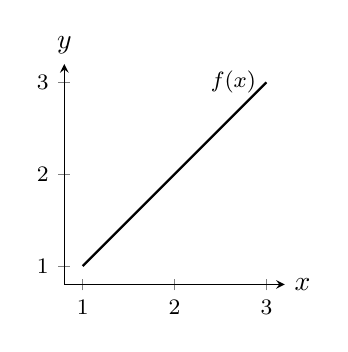
\begin{tikzpicture}[scale=1]
        \begin{axis}[
          axis lines = middle, % boxed, middle
          axis on top,
          axis equal image,
          width=2in,
          %
          % domain and range
          %
          xmin={1}, xmax={3},
          ymin={1}, ymax={3},
          enlargelimits=true,
          %
          % axis labels
          %
          xlabel={\(x\)}, xlabel style={anchor=west},
          ylabel={\(y\)}, ylabel style={anchor=south},
          label style={at={(ticklabel* cs:1)}},
          %
          % ticks
          %
          % xtick={}, xticklabels={},
          % ytick={}, yticklabels={},
          ticklabel style={font=\footnotesize},
          %
          % grid
          % none, major, minor, both
          grid=none, grid style={gray!20},
          % minor tick num=1, 
          % minor grid style={gray!20},
          % 
          % plot parameters
          %
          samples=100, no markers,
          ]
          \addplot[thick] coordinates {(1, 1) (3, 3)} node[left] {\footnotesize \(f(x)\)}; % f(x)
        \end{axis}
      \end{tikzpicture}
      \hspace{0.5in}
      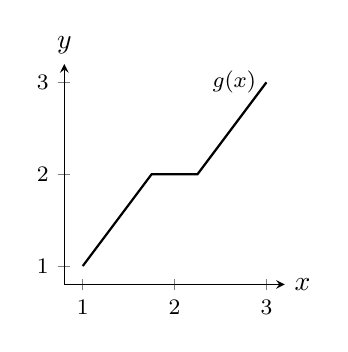
\begin{tikzpicture}[scale=1]
        \begin{axis}[
          axis lines = middle, % boxed, middle
          axis on top,
          axis equal image,
          width=2in,
          %
          % domain and range
          %
          xmin={1}, xmax={3},
          ymin={1}, ymax={3},
          enlargelimits=true,
          %
          % axis labels
          %
          xlabel={\(x\)}, xlabel style={anchor=west},
          ylabel={\(y\)}, ylabel style={anchor=south},
          label style={at={(ticklabel* cs:1)}},
          %
          % ticks
          %
          % xtick={}, xticklabels={},
          % ytick={}, yticklabels={},
          ticklabel style={font=\footnotesize},
          %
          % grid
          % none, major, minor, both
          grid=none, grid style={gray!20},
          % minor tick num=1, 
          % minor grid style={gray!20},
          % 
          % plot parameters
          %
          samples=100, no markers,
          ]
          \addplot[thick] coordinates {(1, 1) (1.75, 2) (2.25, 2) (3, 3)} node[left] {\footnotesize \(g(x)\)}; % g(x)
        \end{axis}
      \end{tikzpicture}
      \hspace{0.5in}
      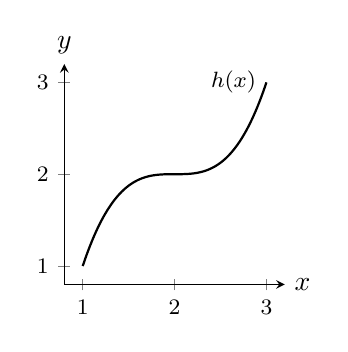
\begin{tikzpicture}[scale=1]
        \begin{axis}[
          axis lines = middle, % boxed, middle
          axis on top,
          axis equal image,
          width=2in,
          %
          % domain and range
          %
          xmin={1}, xmax={3},
          ymin={1}, ymax={3},
          enlargelimits=true,
          %
          % axis labels
          %
          xlabel={\(x\)}, xlabel style={anchor=west},
          ylabel={\(y\)}, ylabel style={anchor=south},
          label style={at={(ticklabel* cs:1)}},
          %
          % ticks
          %
          % xtick={}, xticklabels={},
          % ytick={}, yticklabels={},
          ticklabel style={font=\footnotesize},
          %
          % grid
          % none, major, minor, both
          grid=none, grid style={gray!20},
          % minor tick num=1, 
          % minor grid style={gray!20},
          % 
          % plot parameters
          %
          samples=100, no markers,
          ]
          \addplot[thick, domain=1:3] {(x-2)^3 + 2} node[left] {\footnotesize \(h(x)\)}; % h(x)
        \end{axis}
      \end{tikzpicture}
    \end{center}

    \blanklines{28}
  \end{example}

  \begin{example}
    Review \hlmain{piecewise-defined functions} by reading page 50 and 51 of the textbook pdf.  What questions did you ask yourself? Bring these questions to class next Monday.
  \end{example}
  \clearpage

  Let's more or less follow the textbook order and review linear functions and slopes.

  TODO: talk about rise over run.

  TODO: the standard form of a line is not unique.

  TODO: typo in the definition.
  \clearpage

  We review some common functions (nouns) and operations (verbs) because functions that describe natural phenomena are often created by ``putting together'' basic functions.

  \begin{example}
    Write down one or two examples of the common classes of functions and their general forms.

    \begin{center}
      \begin{tabular}{p{1.25in}p{3.5in}|p{1.5in}}
      & Examples & General Form \\\midrule
        Power \newline functions & & \\[0.75in]\midrule
        Polynomials & & \\[0.75in]\midrule
        Trigonometric \newline functions & & \\[0.75in]\midrule
        Inverse \newline trigonometric \newline functions & & \\[0.75in]\midrule
        Exponential \newline functions & & \\[0.75in]\midrule
        Inverse \newline exponential \newline functions & & \\[0.75in]
      \end{tabular}
    \end{center}
  \end{example}

  \faComments{} Is \(\frac{x^{2}-1}{\sqrt{x-1}}\) a rational function?
    \blanklines{6}
  \clearpage

  Common operations (verbs) on functions \emph{build} sophisticated functions from simpler ones are
  \[
    + \hspace{0.75in}
    - \hspace{0.75in}
    \times \hspace{0.75in}
    \div \hspace{0.75in}
    \circ
  \]
  \blanklines{12}

  \faExclamationTriangle{}
  Note \(f \cdot g\) and \(f \circ g\) are \underline{\hlwarn{not}} (always) the same function!
  \blanklines{5}

  \begin{example} \label{ex:review-circ}
    Suppose \(f(x) = \sqrt{x}\) and \(g(x) = \frac{x^{2}-1}{\sqrt{x-1}}\). Write down \(f \circ g\) and \(g \circ f\).
    \blanklines{20}

    \faComments{} What does Example~\ref{ex:review-circ} teach us about function composition?
    \blanklines{5}
  \end{example}
  \clearpage

  Review of some terminologies. 
  \begin{itemize}[noitemsep]
    \item A \hlmain{root function} is a power function of the form \(x^{1/n}\) or \(\sqrt[n]{x}\) where \(n\) is a \hlsupp{positive} integer. 
      \blanklines[37]{5}

    \item A \hlmain{rational power} is a power function of the form \(x^{p/q}\) where \(p,q\) are integers but \(q \ne 0\).
      \blanklines[37]{5}

    \item Functions that involve \(+, -, \times, \div\), roots and \hlwarn{rational powers} are called \hlmain{algebraic functions}. 
      \blanklines[37]{5}

    \item If a function is \hlsupp{not} algebraic, then it is called a \hlmain{transcendental function}.
      \blanklines[37]{5}

    \item A \hlmain{zero} of a function \(f(x)\) is a \hlsupp{number \(r\)} (in its domain) so that \(f(r) = 0\).  Graphically, zeros of a function are also called its \hlmain{\underline{\hspace{1in}} intercept} or \hlmain{\underline{\hspace{1in}}}.
      \blanklines[37]{5}
  \end{itemize}

  TODO: Discuss why we want to sketch functions by hand.
  % Now we review transformations of functions and a \hlinfo{very general} problem-solving skill:
  % \begin{mdframed}[style=simple]
  %   solve a problem by solving smaller and more manageable problems \hlmain{algebraically}.
  % \end{mdframed}
  % TODO: Explain why we need to know this. Copy and paste textbook table and exercises.
  \clearpage

  Shifting (aka translation) and scaling are two basic types of transformation on functions.

  \hlmain{Shift}: \(f(x + a) + b\) means to move the axes so that the new origin is at the point \((a,b)\).
  \blanklines{20}

  \hlmain{Scale}: \(\beta f(\alpha x)\) means to \hlsupp{scale the \(x\)-axis by \(\alpha\)} but \hlwarn{the graph of \(f(x)\) by \(\beta\)}.
  \blanklines{30}

  \clearpage
  \begin{example}
    Sketch the function \(f(x) = -2\left(\frac{x}{2} + 3\right)^{2}\).
    \blanklines{50}
  \end{example}
\end{lesson}
\end{document}
